\documentclass[sigconf, proceedings, 9pt]{acmart}
\settopmatter{printacmref=false} % Removes citation information below abstract
\renewcommand\footnotetextcopyrightpermission[1]{} % removes footnote with 
%conference information in first column
\usepackage{bigstrut}
\usepackage{amsmath}
\usepackage{balance}
\usepackage{dsfont}
\usepackage{booktabs}
\usepackage{multirow}
\usepackage[english]{babel}
\usepackage{blindtext}
\usepackage{enumitem}
\setlist{leftmargin=*}
\definecolor{Code}{rgb}{.12,.79,.17}
\definecolor{steel}{rgb}{0.4, 0.4,0.7}
\definecolor{Green}{rgb}{.12,.79,.17}
\usepackage{tikz}
\usepackage{calc}
\def\checkmark{\tikz\fill[scale=0.3](0,.35) -- (.25,0) -- (1,.7) -- (.25,.15) 
-- cycle;} 
\def\scalecheck{\resizebox{\widthof{\checkmark}*\ratio{\widthof,{x}}{\widthof{\normalsize
 x}}}{!}{\checkmark}}
%\usepackage[table,dvipsnames]{xcolor}
\usepackage{colortbl}
\newcommand{\gray}{\rowcolor[gray]{.95}}
\pagenumbering{arabic}
\renewcommand{\i}{\item}
\newcommand{\bi}{\begin{itemize}}
\newcommand{\be}{\begin{enumerate}}
\newcommand{\ei}{\end{itemize}}
\newcommand{\ee}{\end{enumerate}}
\newcommand{\tion}[1]{\S~\ref{sect:#1}}
\newcommand{\eq}[1]{Eq.~\ref{eq:#1}}
\newcommand{\fig}[1]{Fig.~\ref{fig:#1}}
\setlength{\abovedisplayskip}{4pt}
\setlength{\belowdisplayskip}{4pt}
\def\bibfont{\small}

\begin{document}
\title{On Recommending Actionable Changes\\For Software Projects}
\author{Rahul Krishna}
\affiliation{NC State University}
\email{i.m.ralk@gmail.com}
%\acmDOI{}
%\acmISBN{}
\acmPrice{}
\acmConference[Fss'17]{}{Foundations of Software Science}{Fall 2017.}{}

\begin{abstract}
Newer generation of software analytics have placed significant emphasis on data 
driven decision making. These decisions are usually based on 
lessons that arise from within a particular project. Some times it is also 
possible to derive these decisions from across multiple projects. In the past, 
research efforts have led to the development of XTREE 
for generating a set of actionable plans within and across projects. We 
postulated that, each of these plans, if followed will improve the quality of 
the software project. Our previous work, however, culminated in an open 
question --- do developers make use of these plans? If so, to what extent?
This work is an attempt to answer these questions. Specifically, we compare the 
overlap between changes made by developers and those recommended by XTREE. To 
this end, we mined several versions of nine popular open source software 
projects. Our results show that recommendations offered by conventional XTREE 
overlaps to an extent of 50\% with changes undertaken by the developers. 
Modified versions of XTREE was developed to improve this overlap. And these 
offer over 75\% overlap.

\end{abstract}

\maketitle

\section{Introduction}
\label{sect:intro}

Over the past decade, advances in AI have enabled a widespread use of data 
analytics in software engineering. For example, we can now estimate how long it 
would take to integrate the new code~\cite{czer11}, where bugs are most likely 
to occur~\cite{Menzies2007a}, or amount of effort it will take to develop a 
software package~\cite{turhan11}, etc. Despite these successes, there is a 
primary operational shortcoming with many software analytic tools lack 
of insightful analytics.

Business users also lament that most software analytics tools, ``Tell us what 
\textit{is}. But they don't tell us 
\textit{what to do}''. A concern that was also raised by several researchers at 
a recent workshop on ``Actionable Analytics'' at 2015 IEEE conference on 
Automated Software Engineering~\cite{hihn15}. For example, most software 
analytics tools in the area of detecting software defects are mostly 
\textit{prediction} algorithms such as Support Vector Machines, Naive Bayes, 
Logistic Regression, Decision Trees, etc~\cite{scikit-learn}. These prediction 
algorithms report what combinations of software project features predict for 
the number of defects. But this is different task to \textit{planning}, which 
answers a more pressing question: what to {\em change} in order to {\em reduce} 
these defects. Accordingly, in this research, we seek tools that offer clear 
guidance on what to do in a specific project.

The tool assessed in this paper is the XTREE \textit{planning} 
tool~\cite{krishna17a}. XTREE employs a $cluster+contrast$ approach to planning 
where it (a) \textit{Clusters} different parts of the software project based on 
a quality measure (e.g. the number of defects); (b) Reports the 
\textit{contrast sets} between neighboring clusters. Each of these contrast 
sets represent the difference between these clusters and they can  be 
interpreted as plans: 
\begin{itemize}
	\item If a current project falls into cluster $C_1$,
	\item Some neighboring cluster $C_2$ has better quality.
	\item Then the difference {\em $\Delta=$ $C_2$ - $C_1$} is a {\em plan} for 
	changing a  project such that it \textit{might} have   higher quality.
\end{itemize}

XTREE uses data from within a software project to these generate plans. 	
Generation of conclusions are an inherent property of XTREE. But, the key 
question with the first version of XTREE is that some of the conclusions were 
not really actionable. So, in this work, we explore ways in which XTREE can 
limit it's conclusions to only actionable ones. 


With this in mind, the rest of this paper is designed as follows. The remainder 
of this
section discusses the research questions asked and answered in this paper. In 
\tion{related}, we discuss the related work in the area of planning in software 
engineering. In \tion{motivate}, we discuss the planning algorithms of this 
paper. The experimental setup is presented in \tion{expt}. The answers to the 
research questions is presented in \tion{results}. We discuss the threats to 
validity of our experiments is discussed in \tion{valid}. Finally, in 
\tion{conclusion}, we present conclusions and directions to future work.

\subsection{Research Questions}
\label{sect:rqs}
\be[leftmargin=-1pt]
\item[] \textbf{\noindent RQ1: How many valid changes does baseline XTREE 
recommend?} 


\textit{Motivation:} The first research question seeks to establish a baseline 
result. Here, we ask how many changes recommended by a simple version of XTREE 
(labeled $XTREE_{simple}$) are actually implemented by developers.


\textit{Approach:} We use a set of 3 datasets -- train, test, validate. We 
construct a planner (XTREE) on the train set, and plan to reduce defects in the 
test set. Then, we look at the validation set, and reflect on the recommended 
changes. We expect to see a number of changes proposed by XTREE to overlap with 
those undertaken by developers. This will also offer us a baseline, which can 
then be improved upon to increase the extent of overlap.


\textit{Results:} We found that with the existing baseline version of XTREE, 
around 50\% of the changes that were recommended by XTREE were also undertaken 
by the developers.


\item[] \textbf{\noindent RQ2: How many defects baseline XTREE assist in 
reducing?}


\textit{Motivation:} In this research question we seek to establish the 
effectiveness of XTREE. That is, for every defective class in the test dataset, 
we look to see if implementing changes recommended by XTREE leads to the 
reduction of defects.


\textit{Approach:} In order to establish this, we look at the defective classes 
in the test dataset, and the same class in the validation dataset. If the 
defects have been fixed, we look to see if the recommendations made by XTREE 
were heeded during that fix. If so, this will point to the uselessness of 
XTREE's plans.

\textit{Results:} We found that XTREE is quite effective in reducing defects. 
In more than 50\% of the cases, the number of defects reduced after using the 
plans proposed by XTREE.


\item[] \textbf{\noindent RQ3: How to extend XTREE to recommend more valid 
changes?} 


\textit{Motivation:} In the first research question, we showed that in 50\% of 
the cases, the plans offered by XTREE were also implemented by developers. In 
this research question, we ask if there is a way to increase the overlap 
between the number of plans proposed by XTREE and those undertaken by 
developers.


\textit{Approach:} To answer this question, we developed two variants of XTREE 
--- $XTREE_{pruned}$ and $XTREE_{all}$. Both the variants use past historical data to modify the plans generated by XTREE in order to ensure that the plans generated are closely related to the changes usually made by developers. The details of their implementation are 
discussed elsewhere in the paper. 


\textit{Results:} Our results show that the modified version of XTREE can 
generate overlaps of upto 80\% with what the developers usually do. This a 
significant improvement to 50\% with the traditional XTREE.


\item[] \textbf{\noindent RQ4: How many defects does extended XTREE assist in 
reducing?} 

\textit{Motivation:} Having demonstrate that $XTREE_{pruned}$ and $XTREE_{all}$ 
can generate samples that are very close to those usually made by developers. 
This research question asks how effective these versions of XTREE are in 
reducing defects.

\textit{Approach:} As for the approach, we take similar steps to RQ2.  We look 
at the defective classes 
in the test dataset, and the same class in the validation dataset. If the 
defects have been fixed, we look to see if the recommendations made by XTREE 
were heeded during that fix. If so, this will point to the uselessness of 
XTREE's plans.


\textit{Results:} Our results indicate that the modified version of XTREE 
performs just as well as the traditional XTREE in all the datasets we have 
studied here.


\ee

\section{Related Work}
\label{sect:related}
Planning  has been a subject of much research in artificial intelligence. Here, 
planning usually refers to generating a sequence of actions that enables an 
\textit{agent} to achieve a specific \textit{goal}~\cite{norvig}. This can be 
achieved by classical search-based problem solving  approaches or logical 
planning agents. Such planning tasks now play a significant role in a variety 
of demanding applications, ranging from controlling space vehicles and robots 
to playing the game of bridge~\cite{ghallab04}. Some of the most common 
planning paradigms include: (a) classical planning~\cite{wooldridge95}; (b) 
probabilistic planning~\cite{altman99}; and (c) preference-based 
planning~\cite{baier09}. 

Existence of a model precludes the use of each of these planning approaches. 
This is a limitation of all these planning approaches since not every domain 
has a reliable model. In software engineering, the planning problem translates 
to proposing changes to software artifacts. Solving this has been undertaken 
via the use of some search-based software engineering 
techniques~\cite{Harman2009}. Examples of algorithms include SWAY, NSGA-II, 
etc.~\cite{nair2016accidental,deb00a}.

These search-based software engineering techniques require access to some 
trustworthy models that can be used to explore novel solutions. In some 
software engineering domains there is ready access to such models which can 
offer assessment of newly generated plans. Examples of such domains within 
software engineering include automated program repair~\cite{Weimer2009, 
LeGoues2015}, software product line management~\cite{sayyad13, henard15}, etc.

However, not all domains come with ready-to-use models. For example, consider 
software defect prediction and all the intricate issues that may lead to 
defects in a product. A model that includes {\em all} those potential issues 
would be very large and complex. Further, the empirical data required to 
validate any/all parts of that model can be hard to find. Also, even when there 
is an existing model, they can require constant  maintenance lest they become 
out-dated. In such domains, we seek alternate methods for planning that can be 
automatically updated with new data without a need for comprehensive models. 
For this, we propose the use of data mining approaches to create a quasi-model 
of the domain 
and make of use observable states from this data to generate an estimation of 
the model. Our preferred tools in this paper (XTREE and BELLTREE) take this 
approach by constructing decision trees on available data (discussed in 
\tion{xtree}). In \tion{results}, we show that these methodologies have 
encouraging results.

In summary, for domains with readily accessible models, we recommend
the tools used by the search-based
software engineering community. For domains, where domain-models are not 
available, we recommend tools such as ours. 


\section{Planning in Software Analytics}
\label{sect:motivate}

In the previous sections, we introduced the notion of planning for decision 
making. In this section we offer a description of each of these planning 
methods:

\subsection{$XTREE_{simple}$}
\label{sect:XTREE}

\begin{figure}[htbp!]
\footnotesize
\centering
\resizebox{.95\linewidth}{!}{
\begin{tabular}{|p{0.95\linewidth}|} \hline
\begin{minipage}{\linewidth}
\small

{\bf \fig{xtree}.A: Top-down division with Decision Trees}

\be
\item Find a split in the values of independent features (OO metrics) that most 
reduces the variability
of the dependent feature (defect counts). For continuous and discrete values,
the {\em variability} can be measured using standard deviation $\sigma$ or 
entropy $e$ respectively. Construct a standard decision tree using these splits.

\item Discretize all numeric features using the Fayyad-Iranni 
discretizer~\cite{fi}
(divide numeric columns into bins $B_i$, each of which  select for the fewest 
cluster ids).
Let feature $F$ have bins $B_i$, each of which contains $n_i$ rows
and let each bin $B_i$ have entropy $e_i$ computed from the frequency of 
clusters seen in that bin.
Cull the the features as per~\cite{papa13}; i.e. just use the $\beta=33\%$ most 
informative features
where  the   value of  feature $F$ is $\sum_i e_i\frac{n_i}{N}$ ($N$ is the 
number of rows).\\[-0.1cm]
\ee
\end{minipage}
\\\hline\textbf{\fig{xtree}.B: A sample XTREE tree.}\\
\begin{minipage}{\linewidth}
% ~\hrule~
\centering
\includegraphics[width=\linewidth]{XTREE_samp.eps}
% ~\hrule~
\end{minipage}\bigstrut\\\hline
\\[-0.2cm]
\begin{minipage}{\linewidth}
\small
% \begin{shaded}  	   

{\small
{\bf \fig{xtree}.C: Using XTREE}

Using the training data,  divide the data using the decision tree algorithm of 
\fig{xtree}.A into groups of
size $\alpha=\sqrt{N}$.
For test item, 
	  find the {\em current } leaf: take each test instance, run it down to a leaf 
	  in the decision tree.  
After that,	  find the {\em desired} leaf:
		\begin{itemize}[leftmargin=3mm]
		\item Starting at {\em current}, ascend the tree $lvl\in \{0,1,2...\}$ levels;
		\item Identify {\em sibling} leaves; i.e. leaf clusters that can be reached 
		from level $lvl$ that are not same as {\em current }
		\item Using the {\em score} defined above, find the {\em better} siblings; 
		i.e. those with a {\em score} less than $\gamma=0.5$ times the mean score of 
		{\em current}. 
		   If none found, then repeat for $lvl += 1$. Also,
		    return no plan if the new $lvl$ is above the root. 
		\item  Return the {\em closest} better sibling where distance is measured 
		between the mean centroids of that sibling and {\em current}
		\end{itemize}
	 Also, find the {\em delta}; i.e. the set difference between  conditions in 
	 the decision tree branch to {\em desired} and {\em current}. To find that 
	 delta: (1)~for discrete attributes, delta is the value from {\em desired}; 
	 (2)~for  numerics, delta is the numeric difference; (3)~for numerics  
	 discretized into ranges, delta is a random number selected from the low and 
	 high boundaries of the that range.
	 
		Finally, return the delta as the plan for improving the test instance.}
% \end{shaded}
\end{minipage}\\\hline
\end{tabular}}
\caption{Generating thresholds using XTREE.}\label{fig:xtree}
\end{figure}

XTREE builds a decision tree,  then generates
plans by contrasting the differences between two branches:
(1)~the branch where you are; (2)~the branch to where you want to be.

XTREE takes a {\em supervised} $Cluster+Contrast$ approach to planning because 
we hypothesize that it is useful to reflect on the target class. Thus, XTREE 
uses a supervised decision tree algorithm of \fig{xtree}.A. To divide 
continuous numeric data, we use a Fayyad-Irani discretizer of \fig{xtree}.B.
Next, XTREE builds plans from the branches of the decision trees using the 
description of \fig{xtree}.C.
In doing so, we ask three questions, the last of which returns the plan:
\be
\item
Which {\em current} branch does a test case fall in?
\item Which {\em desired} branch would the test case want to move to?
\item What are the {\em deltas} between current and desired branches? 
\ee
These \textit{deltas} represent the threshold ranges\footnote{Thresholds are 
denoted by $[low,high)$ ranges for each metric} that represent the plans to 
reduce the defects. 


\subsection{$XTREE_{pruned}$}
$XTREE_{pruned}$ is structurally similar to $XTREE_{simple}$. It differs in the 
steps taken after the construction of the planner. While XTREE uses data from 
the training set to construct a planner, $XTREE_{pruned}$ augments this by 
pruning the branches of the tree by removing the leaves that represent changes 
that have never been seen before. 

To achieve this, we employ first use the past data to keep track of changes 
that were done by developers. Next, we construct XTREE using the same strategy 
as in~\fig{xtree}.  Then, we prune the branches of the tree that represent 
changes that have never been seen before. This pruned tree may then be used to 
generate plans. 

This is a very simple approach. We posit that this will enable us to generate 
plans that not only reduce defects but also increase the likelihood that these 
plans are similar to what developers usually recommend.

\subsection{$XTREE_{all}$}
$XTREE_{all}$ is also structurally similar to $XTREE_{simple}$. It add a few 
additional steps after the construction of the decision tree. We first use data 
from the training set to construct a planner, then for every defective instance 
in the test case, we obtain all possible changes from $XTREE_{simple}$.

Next, we use the past data to keep track of changes that were done by 
developers. Then, we rank the possible changes based on what has previously 
been seen by developers. 

This is also a very simple approach. This ranking process enables us to ensure 
that the generate plans are most likely to reduce defects and also increase the 
likelihood that these plans are similar to what developers usually recommend.

\section{Experimental Setup}
\label{sect:expt}

\subsection{Datasets} 
\label{sect:datasets}
\input{datasets_img.tex}
\begin{figure}[!t]
\scriptsize
\centering
\begin{minipage}{\linewidth}
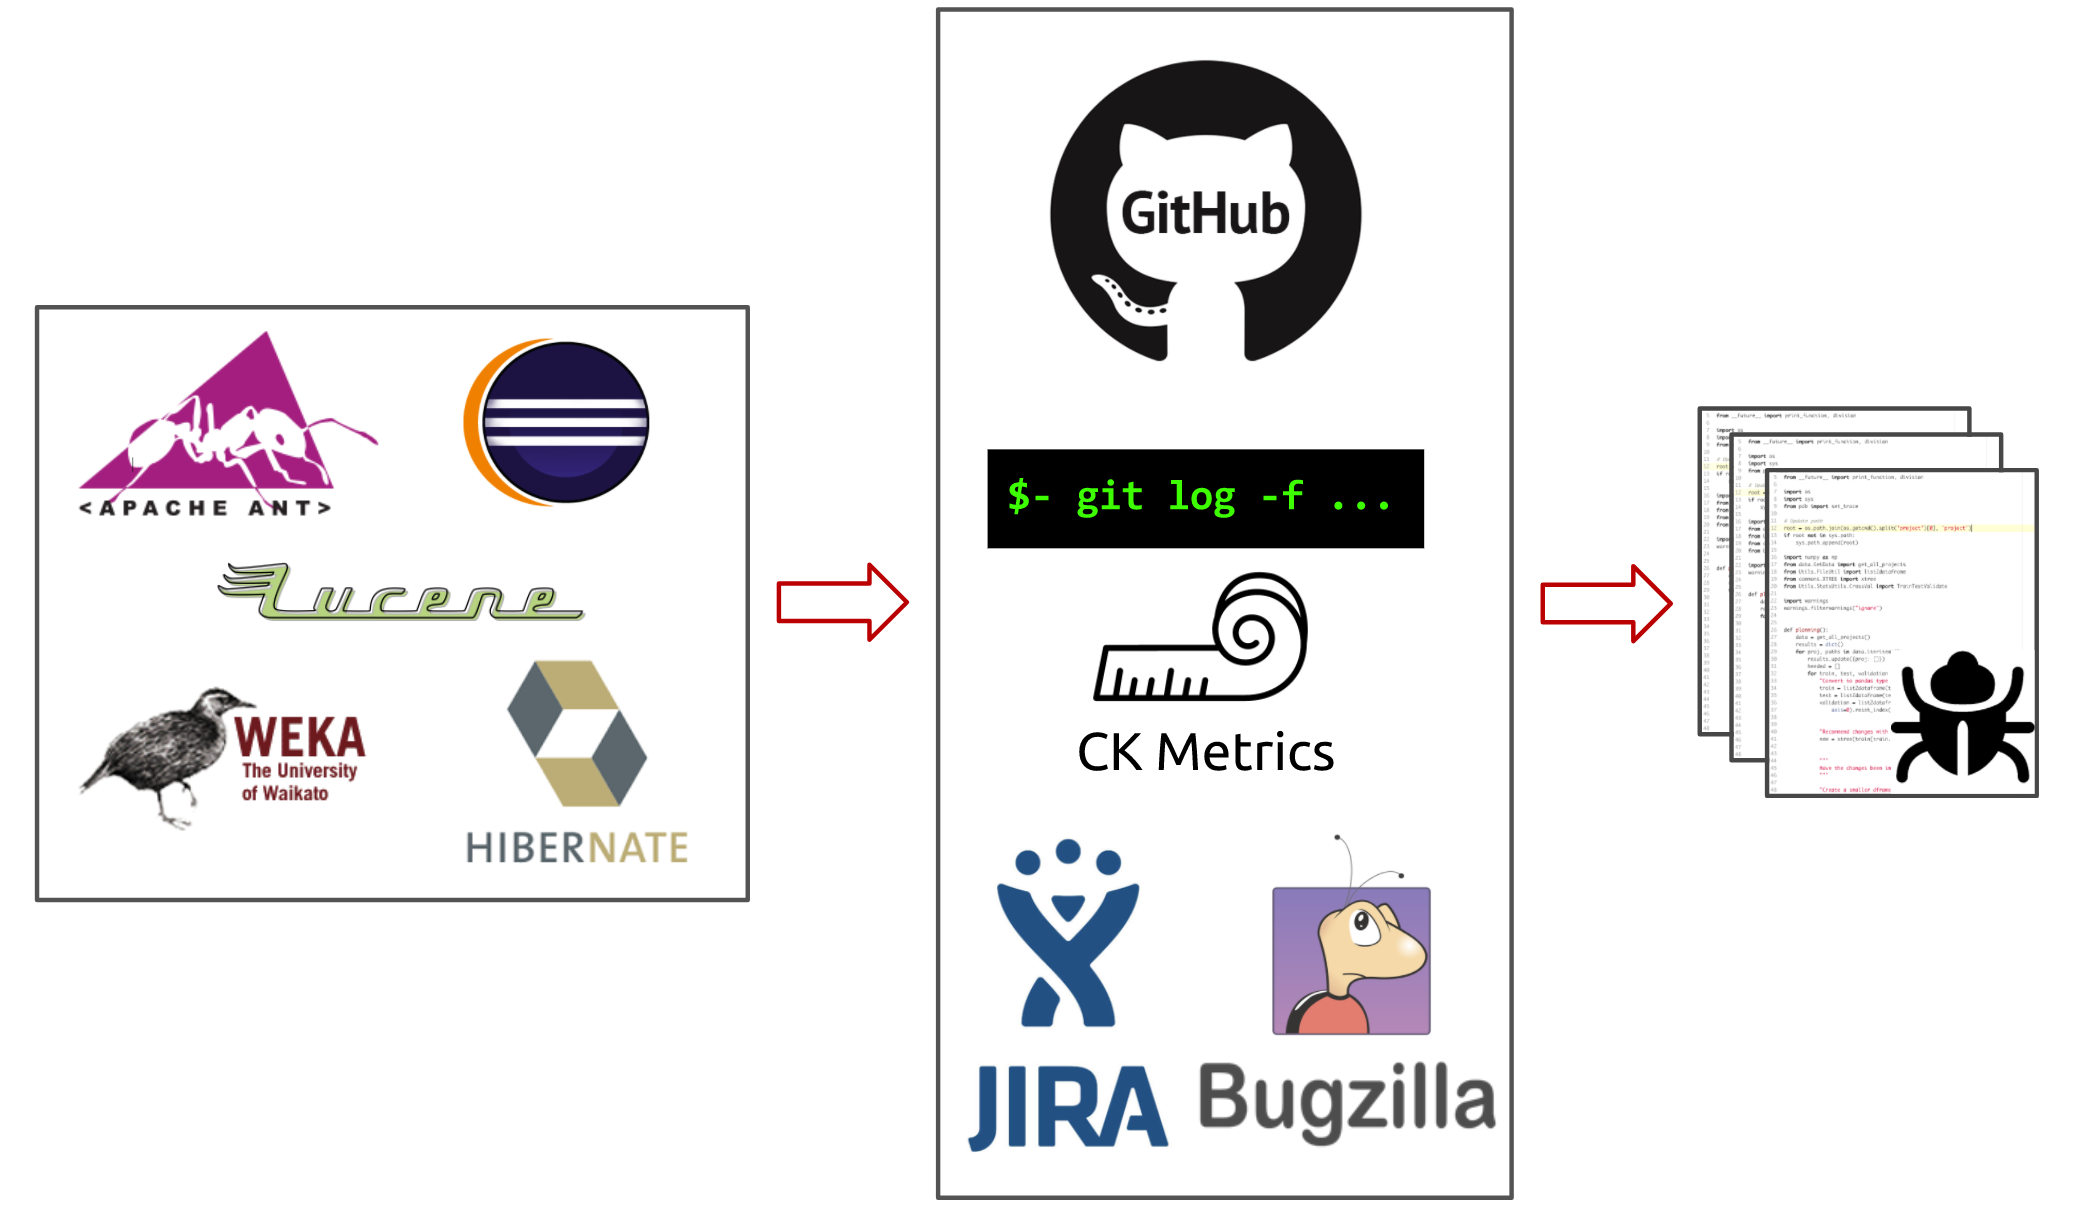
\includegraphics[width=\linewidth]{datasets.png}
\caption{Framework for data generation}\label{fig:datasets1}
\end{minipage}
\begin{minipage}{\linewidth}
\resizebox{\linewidth}{!}{%
% Table generated by Excel2LaTeX from sheet 'Sheet1'
\begin{tabular}{c|l|r|r|r}
\hline
\multirow{2}[4]{*}{Community} & 
\multicolumn{1}{c|}{\multirow{2}[4]{*}{Dataset}} & \multicolumn{3}{c}{\# of 
instances} \bigstrut\\
\cline{3-5}      &       & \multicolumn{1}{r|}{\# Versions} & 
\multicolumn{1}{l|}{\# samples} & Bugs (\%) \bigstrut\\
\hline
\multirow{10}[2]{*}{Java OO} 
& Ant & \multicolumn{1}{r|}{7} & 14289   & 438 (56.01) \\
& Azureus   & \multicolumn{1}{r|}{20} & 25818  & 350 
(20.69) \\
& Ecplise   & \multicolumn{1}{r|}{17} & 978905   & 119 (16.90) \\
& Hibernate & \multicolumn{1}{r|}{38} & 20712 & 303 (17.32) 
\\
& JMeter   & \multicolumn{1}{r|}{8} & 25915  & 707 (51.31) \\
& JStock & \multicolumn{1}{r|}{10} & 59796  & 562 (20.19) \\
& JUnit & \multicolumn{1}{r|}{8} & 25855   & 260 (57.91) \\
& Lucene & \multicolumn{1}{r|}{12} & 58582   & 367 (57.43) \\
& Weka & \multicolumn{1}{r|}{8} & 29816  & 1806 (54.40) \\
\hline
\end{tabular}
}
\end{minipage}
\caption{The figure lists the defect datasets gathered for this project.}
\label{fig:datasets}
\end{figure}
% \begin{figure*}[!t]
% 	\arrayrulecolor{lightgray}
% 	\centering
% 	\resizebox{\linewidth}{!}{%
% 		\begin{tabular}{r|l|l}
% 			wmc & weighted methods per class & \\\hline
% 			dit & depth of inheritance tree & \\\hline
% 			noc &  number of children & \\\hline
% 			cbo & coupling between objects & increased when the methods of one
% 			class access services of another. \\\hline
% 			rfc & response for a class &number of  methods invoked in response to
% 			a message to the object. \\\hline
% 			lcom & lack of cohesion in methods &number of pairs of methods that do
% 			not share a reference to an instance variable. \\\hline
% 			ca & afferent couplings & how many other classes use the specific
% 			class.  \\\hline
% 			ce & efferent couplings & how many other classes is used by the
% 			specific class.  \\\hline
% 			npm & number of public methods &  \\\hline
% 			locm3 & another lack of cohesion measure & if $m,a$ are  the number of
% 			$methods,attributes$
% 			in a class number and $\mu(a)$  is the number of methods accessing an
% 			attribute, 
% 			then
% 			$lcom3=((\frac{1}{a} \sum_j^a \mu(a_j)) - m)/ (1-m)$.
% 			\\\hline
% 			loc & lines of code & \\\hline
% 			dam & data access & ratio of  private (protected)
% 			attributes to   total   attributes \\\hline
% 			moa &  aggregation &  count of the number of data declarations (class
% 			fields) whose types are user defined classes \\\hline
% 			mfa & functional abstraction & number of methods inherited by a class
% 			plus number of methods accessible by member methods of the
% 			class \\\hline
% 			cam & cohesion amongst classes & summation of number of different
% 			types of method parameters in every method divided by a multiplication
% 			of number of different method parameter types in whole class and
% 			number of methods.  \\\hline
% 			ic & inheritance coupling &  number of parent classes to which a given
% 			class is coupled (includes counts of methods and variables inherited)
% 			\\\hline
% 			cbm &coupling between methods &  total number of new/redefined methods
% 			to which all the inherited methods are coupled \\\hline
% 			amc & average method complexity & e.g. number of JAVA byte codes \\\hline
% 			max\_cc & maximum McCabe & maximum McCabe's cyclomatic complexity seen
% 			in class \\\hline
% 			avg\_cc & average McCabe & average McCabe's cyclomatic complexity seen
% 			in class \\\hline
% 			\rowcolor{lightgray}
% 			defect & defect & Boolean: where defects found in post-release 
%bug-tracking systems.
% 		\end{tabular}
% 	} 
% 	\caption{Sample static code attributes.}\label{fig:static_metrics}
% \end{figure*}

\begin{figure*}[tb]
	\renewcommand{\baselinestretch}{0.6}\begin{center}
	{\resizebox{\linewidth}{!}{
			\begin{tabular}{c|l|p{4.7in}}
				amc & average method complexity & e.g. number of JAVA byte codes\\\hline
				avg\, cc & average McCabe & average McCabe's cyclomatic complexity seen
				in class\\\hline
				ca & afferent couplings & how many other classes use the specific
				class. \\\hline
				class. \\\hline
				cam & cohesion amongst classes & summation of number of different
				types of method parameters in every method divided by a multiplication
				of number of different method parameter types in whole class and
				number of methods. \\\hline
				cbm &coupling between methods &  total number of new/redefined methods
				to which all the inherited methods are coupled\\\hline
				cbo & coupling between objects & increased when the methods of one
				class access services of another.\\\hline
				ce & efferent couplings & how many other classes is used by the
				specific class. \\\hline
				dam & data access & ratio of the number of private (protected)
				attributes to the total number of attributes\\\hline
				dit & depth of inheritance tree &\\\hline
				ic & inheritance coupling &  number of parent classes to which a given
				class is coupled (includes counts of methods and variables inherited)
				\\\hline
				lcom & lack of cohesion in methods &number of pairs of methods that do
				not share a reference to an case variable.\\\hline
				locm3 & another lack of cohesion measure & if $m,a$ are  the number of
				$methods,attributes$
				in a class number and $\mu(a)$  is the number of methods accessing an
				attribute, 
				then
				$lcom3=((\frac{1}{a} \sum, j^a \mu(a, j)) - m)/ (1-m)$.
				\\\hline
				loc & lines of code &\\\hline
				max\, cc & maximum McCabe & maximum McCabe's cyclomatic complexity seen
				in class\\\hline
				mfa & functional abstraction & number of methods inherited by a class
				plus number of methods accessible by member methods of the
				class\\\hline
				moa &  aggregation &  count of the number of data declarations (class
				fields) whose types are user defined classes\\\hline
				noc &  number of children &\\\hline
				npm & number of public methods & \\\hline
				rfc & response for a class &number of  methods invoked in response to
				a message to the object.\\\hline
				wmc & weighted methods per class &\\\hline
				\rowcolor{lightgray}
				nDefects & raw defect counts & Numeric: number of defects found in 
				post-release bug-tracking systems.\\
				\rowcolor{lightgray}
				isDefective & defects present? & Boolean: if {\em nDefects} $>0$ then {\em 
				true} else {\em false}
			\end{tabular}}
			}
	\end{center}
	\caption{OO code metrics used for all studies in this paper.
	   Last lines, shown in \textcolor{gray}{gray}, denote the dependent 
	   variables.}\label{fig:static_metrics}
\end{figure*}

The defect dataset used in this study comprises a total of 9 datasets that were 
mined from GitHub. The projects primarily involve systems developed in JAVA. 
For these systems, we measure defects at class and method-level granularity. 

The procedure used to mine these datasets is illustrated in 
\fig{datasets1}. All the datasets are 
described in terms of the attributes of \fig{static_metrics}. In order to 
gather these datasets, we use the following steps:
\be
\item Find the most popular JAVA projects on GitHub. For these projects, clone 
them locally and generate a complete log of release dates and commit messages.
\item For each release, build the project and gather the CK-Metrics. We used 
the ckjm tool\footnote{https://github.com/mjureczko/CKJM-extended} for this.
\item Use the commit messages between each releases to identify ``bug-fixing'' 
commits.
\item For each ``bug-fixing'' commit, find the respective files that are 
changed and mark them as defect prior to the release.
\ee

The above process, when repeated for all the projects, generates the required 
datasets. In \fig{datasets}, we summarize all the datasets that were mined for 
experimentation. All these datasets records the number of known defects 
for each class using a post-release bug tracking system. The classes are 
described in terms of 20 OO metrics, including CK metrics and McCabes 
complexity metrics. 


\subsection{Evaluation Strategy}
\label{sect:procedure}
\begin{figure}
\centering
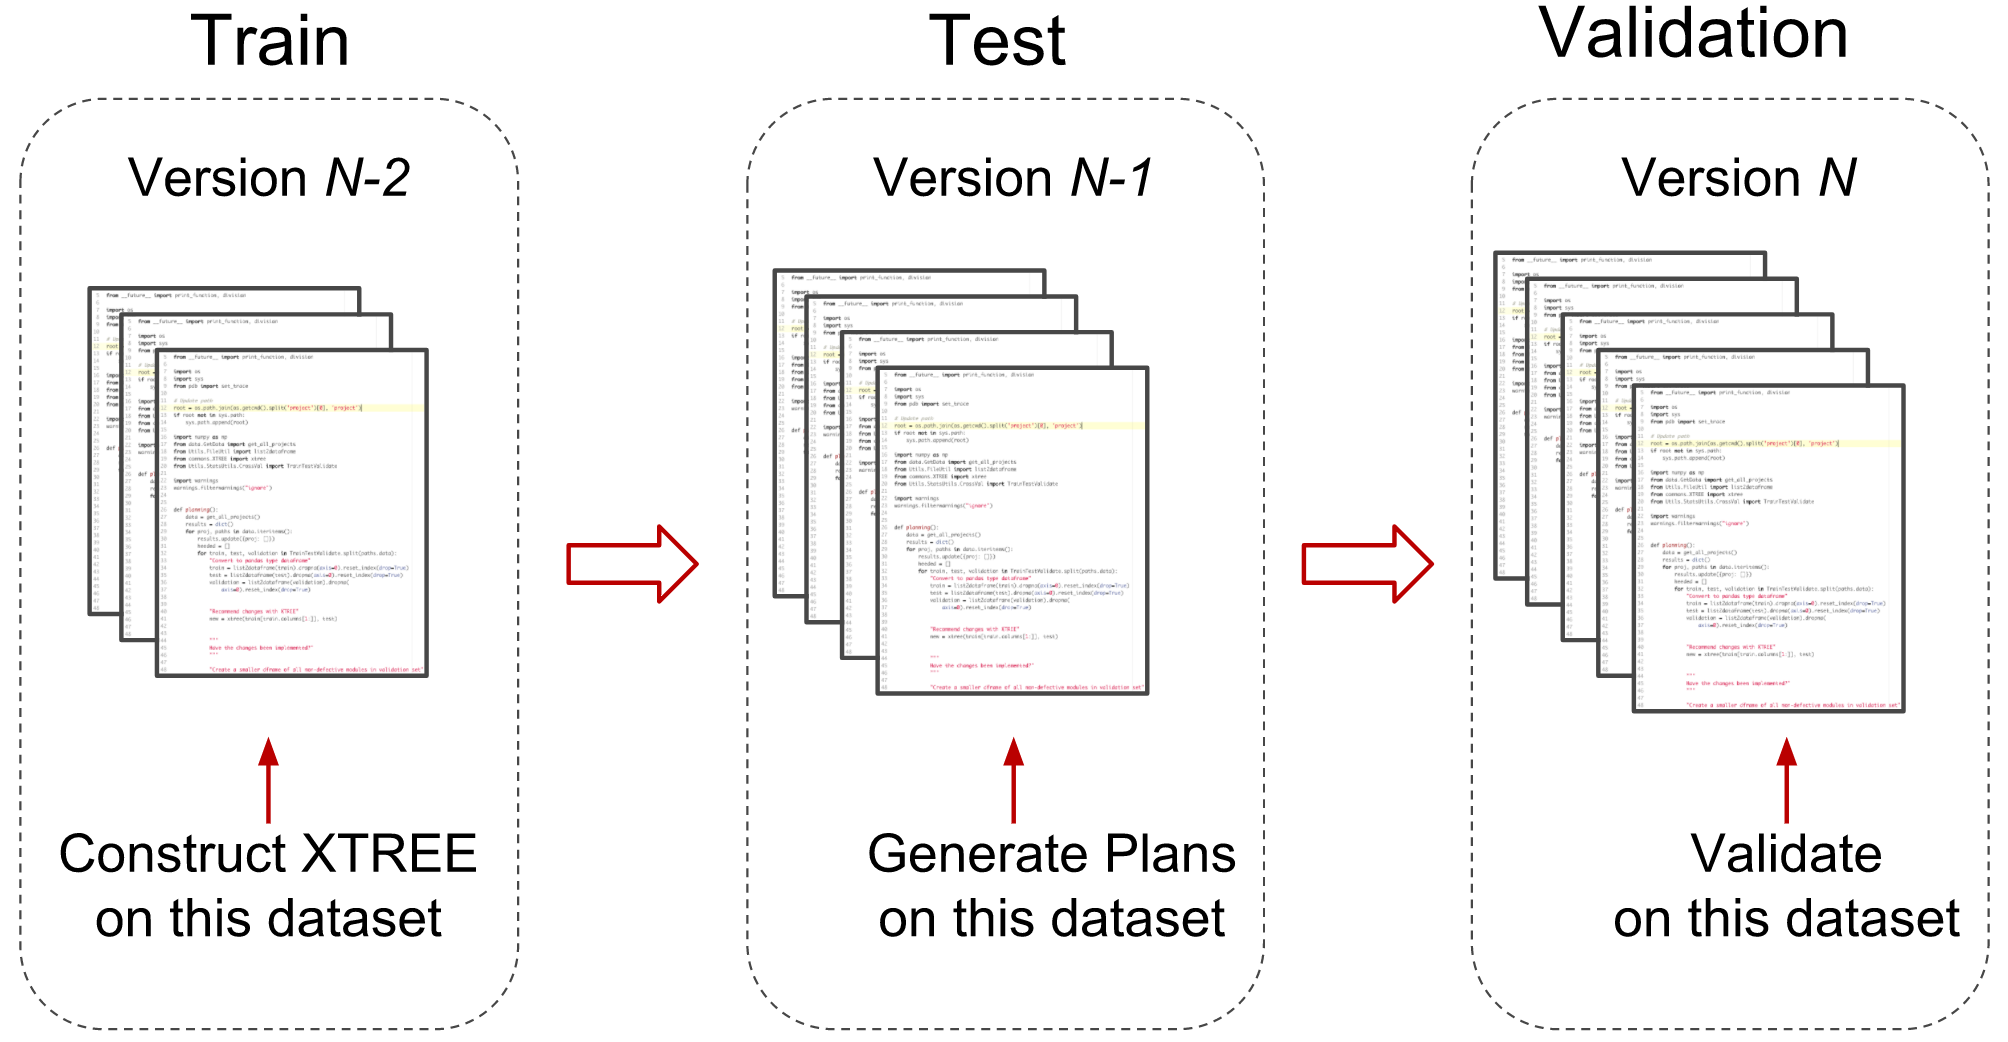
\includegraphics[width=\linewidth]{expt_design.png}
 \caption{Experimental design}\label{fig:design}
\end{figure}

Our experimental design is shown in \fig{design}. For a project $\mathbb{P}$ 
with versions $\mathcal{V}=\{1, ..., N\}$, we divide the
project data  into three parts: we use $\mathcal{V}-2$ as the \textit{train 
set}, $\mathcal{V}-1$ as the \textit{test test}, and $\mathcal{V}$ as the
\textit{validation set} in the following fashion:

\be
\item The train test is used to construct the planner. In \tion{planners} we 
describe the planners and a way to translate these plans 
into actionable decisions. 
\item Next, the test set used to generate for. That is, for every defective 
module in the test set, we obtain plans from the train set.
\item The validation set is used to assess the effect of acting on these plans. 
This is necessary because it lets us judge the  effects of applying the plan. 
If the defect has been fixed in the validation set as a result of complying 
with plans from XTREE.
\ee

The above steps are repeated for all the $N$ versions of every project. 

In software analysis, there is the issue of reliable verification oracles to 
test effects of planning. To resolve this problem, SE researchers such as
Cheng et al.~\cite{Cheng10}, O'Keefe et al.~\cite{OKeeffe08,OKeeffe07},
Moghadam~\cite{Moghadam2011} and Mkaouer et al.~\cite{Mkaouer14}
use a {\em verification oracle} that is learned separately
from the primary oracle. The verification oracles assesses
how defective the code is before and after some
code changes.
For their verification oracle,
Cheng, O'Keefe, Moghadam and  Mkaouer et al. use the QMOOD hierarchical
quality model~\cite{Bansiya02}.
A shortcoming of QMOOD
is that quality models learned from other projects
may perform poorly when applied to new projects~\cite{localvsglobal}.

Hence, for this study, we make use of the validation set in place of 
verification oracle. These validation sets represent the ground truth and are 
therefore a true representation of the impact of acting on these plans.

\subsection{Performance Measures}
\label{sect:evaluation}

\subsubsection{Effectiveness}
\label{sect:effectiveness}
For planning and construction of a verification oracle, we divide the
project data into two parts the \textit{train set} and the \textit{test test}.
The train set could either be data that is available locally within a project, 
or it could be data from the bellwether dataset. We further partition the train 
set to build both a {\em planner} and a {\em verification oracle}. Note that: 
{\em The verification oracle should be built with completely different data to 
the planner.}

After constructing the planner and verification oracle, we (1)~deploy the 
{planner} to recommend plans; (2)~alter the {\em test} data according to these 
plans;
then (3)~apply the {verification oracle} to the altered data to estimate 
defects; then (3)~Compute the percent improvement, denoted by the following 
equation:
\begin{equation}
\small
\label{eq:effectiveness}
R=(1-\frac{\mathit{after}}{\mathit{before}})\times100\%
\end{equation}
The value of the measure $R$ has the following properties: (1) If $R = 0\%$, 
this means  ``no change from baseline''; 
(2) If $R > 0\%$, this indicates ``improvement'';
(3) If $R < 0\%$, this indicates ``optimization failure''. Ideally, an 
effective planner should have an improvement of $R>0$, where larger values 
indicate better performance. 
\subsubsection{Overlap}
\label{overlap} In order to measure the number of changes common to what the 
developers implemented and what XTREE recommends, we use a measure called 
overlap. Overlap is given as follows:
\begin{equation}
\label{eq:overlap}
O = \left(\frac{{XTRE{E_{recommended}}}}{{Changed}} + \frac{{XTRE{E_{not - 
recommended}}}}{{Unchanged}}\right)\times100
\end{equation}
Where, $XTRE{E_{recommended}}$ is the changes recommended by XTREE, $Changed$ 
are the changes implemented by the developers. Similarly, $XTRE{E_{not - 
		recommended}}$ are the changes not-recommended by developers and $Unchanged$ 
		are the change not-performed by the developer. The higher the value of 
		overlap between XTREE's recommendations and the actual changes performed by 
		the developers, the larger the value of $O$
\subsection{Statistics}
\label{sect:stats}
Changes made to module in a software project are subject to inherent 
randomness. Researchers have endorsed the use of repeated runs 
to gather reliable evidence~\cite{vaux2012replicates}. Thus, we repeat the 
whole experiment independently using a moving window over 
the various versions  of the project (see \tion{procedure}) to provide evidence 
that the results are reproducible. These repeats provide us with a sufficiently 
large sample size to statistically compare the performances. 

At each position of the moving window, we collect the values of effectiveness R 
(\eq{effectiveness})
and overlap O (\eq{overlap}). We refrain from 
performing a cross validation because the process tends to mix the samples 
from training data (the source) and the test data (other target 
projects), which defeats the purpose of this study.

To rank the numbers collected above, we use the Scott-Knott test 
recommended by Mittas and Angelis~\cite{mittas13}. Scott-Knott is a 
top-down clustering approach used to rank different treatments. If that 
clustering finds an statistically significant splits in data, then some 
statistical test is applied to the two divisions to check if they are 
statistically significant different. If so, Scott-Knott recurses into both 
halves.

To  apply Scott-Knott, we sorted a list of  $l$ values of \eq{G} 
values found in $ls$ different methods. Then, we split $l$ into 
sub-lists $m,n$ in order to maximize the expected value of differences in 
the observed performances before and after divisions. E.g. for lists 
$l,m,n$ of size $ls,ms,ns$ where $l=m\cup n$: 
\[E(\Delta)=\frac{ms}{ls}abs(m.\mu - l.\mu)^2 + \frac{ns}{ls}abs(n.\mu - 
l.\mu)^2\] 


We then apply a statistical hypothesis test $H$ to check
if $m,n$ are significantly different. In our case, the conjunction of 
bootstrapping and A12 test. Both the techniques are non-parametric in nature, 
i.e., they do not make gaussian assumption about the data. As for hypothesis 
test, we use a non-parametric bootstrapping test as endorsed by Efron \& 
Tibshirani~\cite[p220-223]{efron93}. Even with statistical significance, it is 
possible that the difference
	can be so small as to be of no practical value. This is known as a ``small 
	effect''. To ensure that the statistical significance is not due to ``small 
	effect'' we use effect-size tests in conjunction with hypothesis tests. A 
	popular effect size test used in SE literature is the A12 test. It has been 
	endorsed by several SE researchers~\cite{leech2002call, poulding10, arcuri11, 
	shepperd12a, kampenes07, Kocaguneli2013:ep}. It was first proposed by Vargha 
	and Delany~\cite{vargha2000}. In our context,
	given the performance measure 
	G, the A12 statistics measures the
	probability that one treatment yields higher $G$ values than another. If the 
	two algorithms are equivalent, then A12 = 0.5. Likewise if $A12 \ge 0.6$, then 
	60\% of the times, values of one treatment are significantly greater that the 
	other. In such a case, it can be claimed that there is \textit{significant 
	effect} to justify the hypothesis test $H$. In our case, we divide the data if 
	\textit{both} bootstrap sampling and effect size test agree that a division is 
	statistically significant (with a
	confidence of 99\%) and not a small effect ($A12 \ge 0.6$). Then, we recurse 
	on each of these splits to rank G-scores from best to worst.




\section{Results}
\label{sect:results}

\subsection*{\textbf{RQ1: How many valid changes does baseline XTREE 
recommend?}}
\begin{figure}[t]
\centering
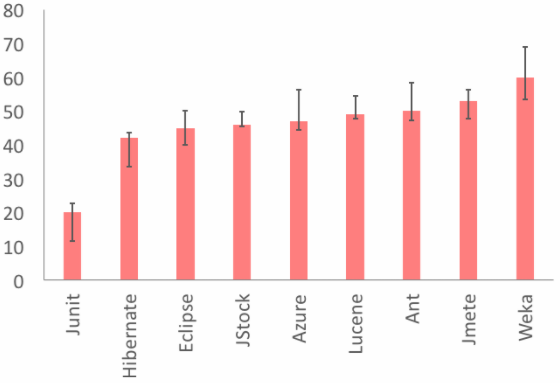
\includegraphics[width=\linewidth]{rq1.png}
\caption{Overlap between changes implemented by developers and those 
recommended by XTREE.}
\label{fig:rq1}
\end{figure}

The purpose of this research question was to establish a baseline result. Here 
we use XTREE to recommend plans for addressing classes with defects. Then we 
compare those recommended plans with the changes undertaken by developers to 
fix those defects. Finally, we compare the overlap between the recommendations 
offered by XTREE with those undertaken by developers using \eq{overlap}.

Our results are shown in \fig{rq1}. In the figure, we see that plans generated 
$XTREE_{simple}$ overlap with the developer's fixes by about 50\%. That is in 
50\% of the cases, the recommendations of XTREE is the same as those done by 
developers. The results are quite encouraging because they offer a number of 
possibilities for improvement.

\subsection*{\textbf{RQ2: How many defects baseline XTREE assist in 
reducing?}}
\subsection*{\textbf{RQ3: How to extend XTREE to recommend more valid 
changes?}} 
\subsection*{\textbf{RQ4: How many defects does extended XTREE assist 
in reducing?}} 

\section{Reliability and Validity of Conclusions}
\label{sect:valid}



The results of this paper are biased by our choice of code reorganization
goal (reducing defects) and our choice of measures collected from software
project (OO measures such as depth of inheritance, number of child classes,
etc). That said, it should be possible extend the methods of this paper to 
other
kinds of goals (e.g. maintainability, reliability, security, or the 
knowledge sharing
measures) and other kinds of
inputs (e.g. the process measures favored by Rahman,
Devanbu et al.~\cite{Rahman2013})

\subsection{Reliability}
Reliability refers to the consistency of the results obtained
from the research. It has at least two components: internal
and external reliability.

Internal reliability checks if an independent researcher
reanalyzing the data would come to the same conclusion.
To assist other researchers exploring this point, we offer a full 
replication package for this study at
https://github.com/rahlk/FSS17.

External reliability assesses how well independent researchers
could reproduce the study. To increase external
reliability, this paper has taken care to clearly define our
algorithms. Also, all the data used in this work is available
online.

For the researcher wishing to reproduce our work to other kinds of goals, 
we offer the following advice:

\begin{itemize}
\item Find a data source for the other measures of interest;
\item Implement another secondary verification oracle that can assess 
maintainability, reliability, security, technical debt, etc;
\item Implement a better primary verification oracle that can do ``better'' 
than XTREE at finding changes (where ``better'' is defined in terms
of the opinions of the verification oracle). 
\end{itemize}


\subsection{Validity}

This paper is a case study that studied the effects of  limiting 
unnecessary code reorganization on some data sets. This section discusses 
limitations of such case studies. In this context, validity refers to the 
extent to which a piece of research actually
investigates what the researcher purports to investigate.
Validity has at least two components: internal and
external validity.


Based on the case study presented above,
as well as the discussion in \tion{prelim},
we believe that defect indicators (e.g. \mbox{{\em loc}$>$ 100})
have limited external validity beyond the projects from which they are 
derived.
While specific models are externally valid,
there may still be general methods like XTREE for finding the good local 
models.

Our definition of bad smells is limited to those represented by OO code 
metrics (a premise often used in related work).
XTREE, Shatnawi, Alves et al. can  only comment
on bad smells   expressed as code metrics
in the historical log of a project.

If developers want to justify their code reorganizations
via bad smells expressed in other terminology,
then the  analysis of this paper must:
\begin{itemize}
	\item Either wait till
	data about those new
	terms has been collected.
	\item Or, apply cutting edge transfer learning
	methods~\cite{Nam15,Jing15, krishna16} to map data from other projects
	into the current one.
\end{itemize}
Note that the transfer learning approach would
be highly experimental and require more study
before it can be safely recommended.

Sampling bias threatens any data mining analysis; i.e., what matters
there may not be true here. For example, the data sets used here comes 
from 
Jureczko et al. and any biases in their selection procedures
threaten the validity of these results.
That said,
the best we can do is define our methods and publicize our data and code so 
that other researchers can
try to repeat our results and, perhaps, point out a previously unknown bias
in our analysis. Hopefully, other researchers will emulate our methods in
order to repeat, refute, or improve our results.


\section{Conclusions and Future Work}
\label{sect:conclusion}


\balance
\bibliographystyle{ACM-Reference-format}
\bibliography{final}
\end{document}
